\begin{figure}[ht]
% \vskip 0.2in
\begin{center}
\centerline{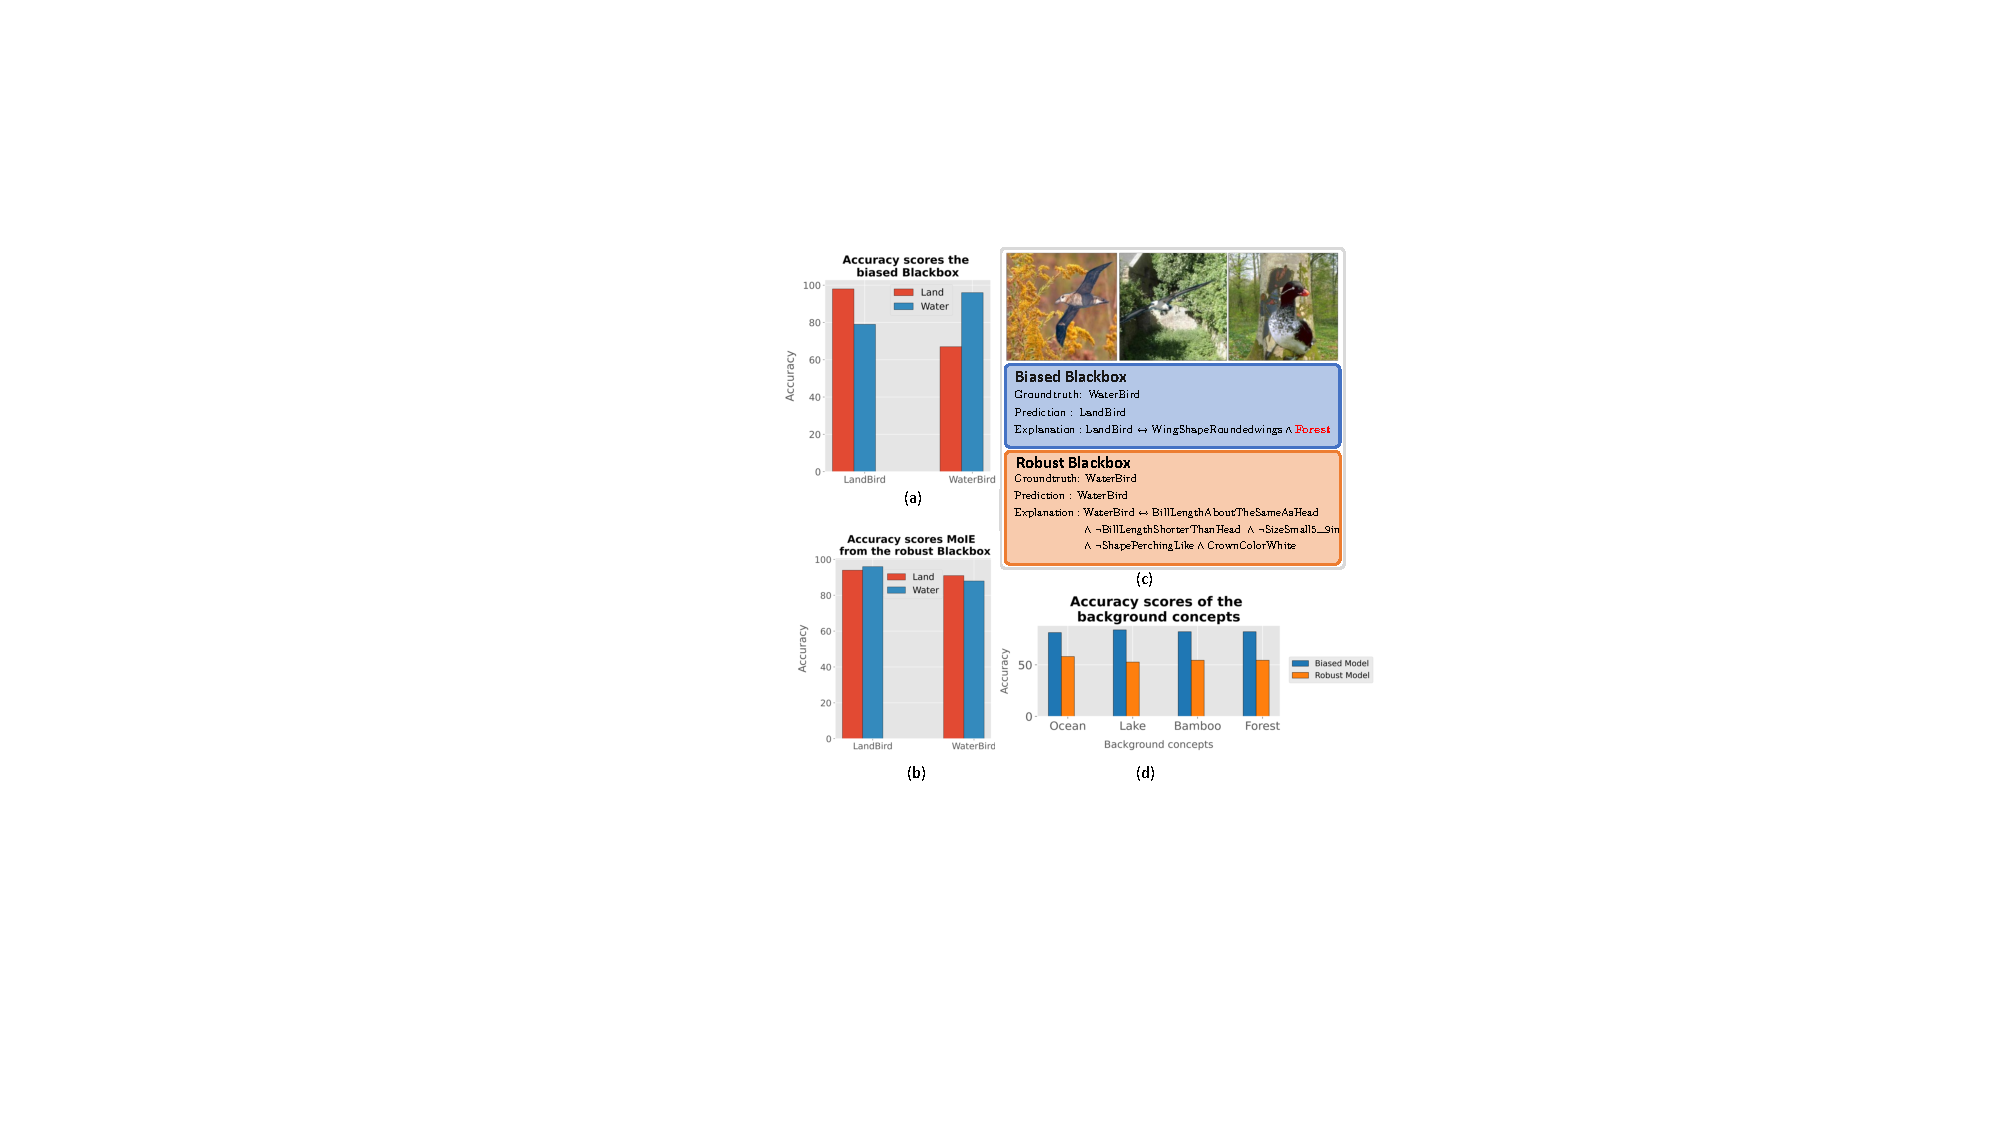
\includegraphics[width=\columnwidth]{figures/main/shortcut.pdf}}
\caption{MoIE fixes shortcuts. \textbf{(a)} Performance of the biased Blackbox. 
\textbf{(b)} Performance of final MoIE extracted from the robust Blackbox after removing the shortcuts using MDN. 
\textbf{(c)} Examples of samples (\textbf{top-row}) and their explanations by the biased (\textbf{middle-row}) and robust Blackboxes (\textbf{bottom-row}). 
\textbf{(d)} Comparison of accuracies of the spurious concepts extracted from the biased vs. the robust Blackbox.
}
\label{fig:shortcut}
\end{center}
\vskip -0.2in
\end{figure}

First, we create the Waterbirds dataset as in~\cite{sagawa2019dro}by using forest and bamboo as the spurious land concepts of the Places dataset for landbirds of the CUB-200 dataset. We do the same by using oceans and lakes as the spurious water concepts for waterbirds. We utilize ResNet50 as the Blackbox $f^0$ to identify each bird as a Waterbird or a Landbird. The Blackbox quickly latches on the spurious backgrounds to classify the birds. As a result, the black box's accuracy differs for land-based versus aquatic subsets of the bird species, as shown in~\cref{fig:shortcut}a. The Waterbird on the water is more accurate than on land (96\%  vs. 67\% in the red bar in the~\cref{fig:shortcut}a). The FOL from the biased Blackbox-derived MoIE captures the spurious concept \textit{forest} for a waterbird, misclassified as a landbird. Assuming the background concepts as metadata, we remove the background bias from the representation of the Blackbox using Metadata normalization (MDN) layers~\cite{lu2021metadata} between two successive layers of the convolutional backbone to fine-tune the biased Blackbox to make it more robust. Next, we train $t$, using the embedding $\Phi$ of the robust Blackbox, and compare the accuracy of the spurious concepts with the biased blackbox in~\cref{fig:shortcut}d. The validation accuracy of all the spurious concepts retrieved from the robust Blackbox falls well short of the predefined threshold 70\% compared to the biased Blackbox. Finally, we re-train the MoIE distilling from the new robust Blackbox.~\cref{fig:shortcut}b illustrates similar accuracies of MoIE for Waterbirds on water vs. Waterbirds on land (89\% - 91\%). The FOL from the robust Blackbox does not include any background concepts (~\ref{fig:shortcut}c, bottom row). Refer to~\ref{fig:spurious_flow} in~\cref{app:shortcut} for the flow diagram of this experiment.